\documentclass[11pt, convert={outext=.png}]{standalone}
\usepackage{tikz}
\usetikzlibrary{math}
\usepgflibrary{patterns.meta}
\usetikzlibrary{patterns.meta}
\begin{document}
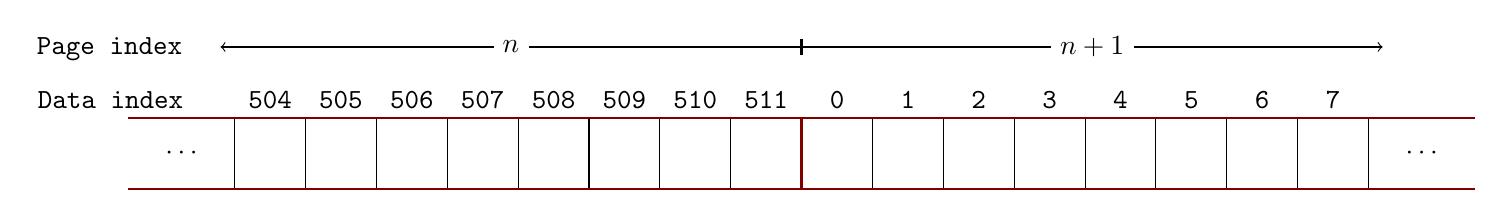
\begin{tikzpicture}
	% Constants
	\tikzmath{
		int \numrect, \totalrect, \dataindex;
		\numrect = 8; \totalrect = int(2 * \numrect);
		\datawidth = 0.9; \dataheight=0.9; \textstagger=-0.30;
	}

	\begin{scope}
		\foreach \i [
			% Each data point
			evaluate=\i as \drawcoord using (\i - \numrect - 1) * \datawidth,
			% Indices associated with point
			evaluate=\i as \nodecoord using (\i - \numrect - 0.5) * \datawidth,
			evaluate=\i as \dataindex using {int(mod(int(\i + 511 - \numrect), 512))},
		] in {1, 2, ...,  \totalrect} {
				% Box for point
				\draw (\drawcoord, 0) rectangle ++(\datawidth, \dataheight);
				% Indices associated with box
				\node[anchor=south] at (\nodecoord, \dataheight) {\texttt{\dataindex}};
			}

		% Page delimiter
		\draw[thick, red!50!black, draw opacity=1.0] ({ -(\numrect + 1.5) * \datawidth }, 0) -- (0, 0) -- (0, \dataheight) -- ({ -(\numrect + 1.5) * \datawidth }, \dataheight);
		\draw[thick, red!50!black, draw opacity=1.0] ({ (\numrect + 1.5) * \datawidth }, 0) -- (0, 0) -- (0, \dataheight) -- ({ (\numrect + 1.5) * \datawidth }, \dataheight);
		% Additional data points
		\node[anchor=center] at ({-(\numrect + 0.75)*\datawidth}, \dataheight/2) {$\cdots$};
		\node[anchor=center] at ({ (\numrect + 0.75)*\datawidth}, \dataheight/2) {$\cdots$};
		% Data index
		\node[anchor=335] at ({-(\numrect + 1.2)*\datawidth}, \dataheight) {\texttt{Data index}};
		% Page index
		\draw[|->] (0, {\dataheight-3*\textstagger}) -- ++({-(\numrect + 0.2)*\datawidth}, 0) node[midway, anchor=center, fill = white] {$n$};
		\node[anchor=332] at ({-(\numrect + 1.2)*\datawidth}, {\dataheight-2*\textstagger}) {\texttt{Page index}};
		\draw[|->] (0, {\dataheight-3*\textstagger}) -- ++({ (\numrect + 0.2)*\datawidth}, 0) node[midway, anchor=center, fill = white] {$n+1$};
	\end{scope}
\end{tikzpicture}
\end{document}
